% Revisado
\subsection{Contexto Histórico e Econômico}

    A prática sistemática de classificação do algodão remonta ao início do século XIX, tendo Liverpool (Inglaterra) como berço comercial. A implementação dessa padronização foi uma resposta direta à Primeira Revolução Industrial: com a modernização das máquinas de fiar, observou-se que a eficiência produtiva e a qualidade do fio dependiam intrinsecamente da uniformidade da fibra, impactando a margem de lucro do setor têxtil \cite{morais2021interpretacao}. Inicialmente, a percepção de qualidade variava conforme o agente (produtor ou indústria), gerando assimetria de informações. A criação de uma terminologia padronizada e de critérios objetivos tornou-se, portanto, essencial para garantir uma base de comparação justa nas transações internacionais \cite{earle1914classification}.

    Nos Estados Unidos, um marco regulatório foi a adoção do \textit{United States Cotton Futures Act} pela Bolsa de Algodão de Nova York, conforme discutido por \citeonline{conant1915us}. Essa legislação substituiu o sistema arbitrário de diferenciação de preços por um modelo baseado nas diferenças comerciais reais do mercado à vista (\textit{spot market}). O ato tinha como objetivo alinhar os contratos futuros à realidade do mercado físico, mitigando distorções que prejudicavam o \textit{hedge} e a confiança dos investidores. Além disso, introduziu a supervisão governamental na identificação dos fardos, trazendo transparência ao processo.

    Segundo \citeonline{earle1914classification}, o sistema oficial de classificação estadunidense foi consolidado no início do século XX pelo Departamento de Agricultura (\textit{United States Department of Agriculture} - USDA), resultando nos Padrões Físicos Universais. A partir da década de 1960, o USDA impulsionou o desenvolvimento de métodos instrumentais, culminando na adoção massiva do sistema HVI. Atualmente, embora a classificação instrumental seja predominante na produção estadunidense, a inspeção visual manual ainda é utilizada para identificação de contaminantes específicos, sendo objeto de pesquisas contínuas para a automação total do processo \cite{knowlton2005usda, cottoninc2020classification}.


\subsection{Métodos e Padrões de Classificação no Brasil}

    No Brasil, a classificação da pluma é regida pela Instrução Normativa n.º 24/2016 do Ministério da Agricultura, Pecuária e Abastecimento (MAPA). O regulamento harmoniza os procedimentos nacionais aos Padrões Físicos Universais, avaliando atributos como cor, presença de folhas, impurezas, contaminação de matérias estranhas e o modo de beneficiamento \cite{mapa2016}.

    O processo tem início com uma amostragem rigorosa para garantir a representatividade do lote. Conforme a normativa, devem ser extraídas duas amostras de lados opostos de cada fardo (mínimo de 150g cada). Estas são divididas longitudinalmente e combinadas para formar as amostras de trabalho: uma destinada à classificação visual e outra à instrumental. As dimensões (25 a 30 cm de comprimento) e o acondicionamento devem assegurar que a estrutura da pluma não seja descaracterizada antes da análise.

    \clearpage

    \subsubsection{A Classificação Visual}

        A classificação visual é realizada por técnicos habilitados, os classificadores, que utilizam como referência os Padrões Físicos Universais (\textit{Universal Standards}). Esses padrões, estabelecidos pelo USDA e adotados no Brasil, consistem em caixas contendo amostras físicas de algodão que representam as classes de cor e graus de folha (\textit{Leaf Grade}) para as variedades \textit{Upland} e \textit{Pima}\footnote{No Brasil, especialmente no cerrado mato-grossense cultiva-se quase que exclusivamente o algodão Upland (\textit{Gossypium hirsutum}). O algodão Pima (\textit{Gossypium barbadense}) é típico do Peru, Egito e EUA.}, conforme ilustrado na Figura \ref{fig_padrao_fisico}.

        \begin{figure}[H]
            \caption{\label{fig_padrao_fisico}Exemplo do Padrão Físico Universal (51.5: Cor Abaixo da Média, Branco / Grau de Folhas 5)}
            \begin{center}
                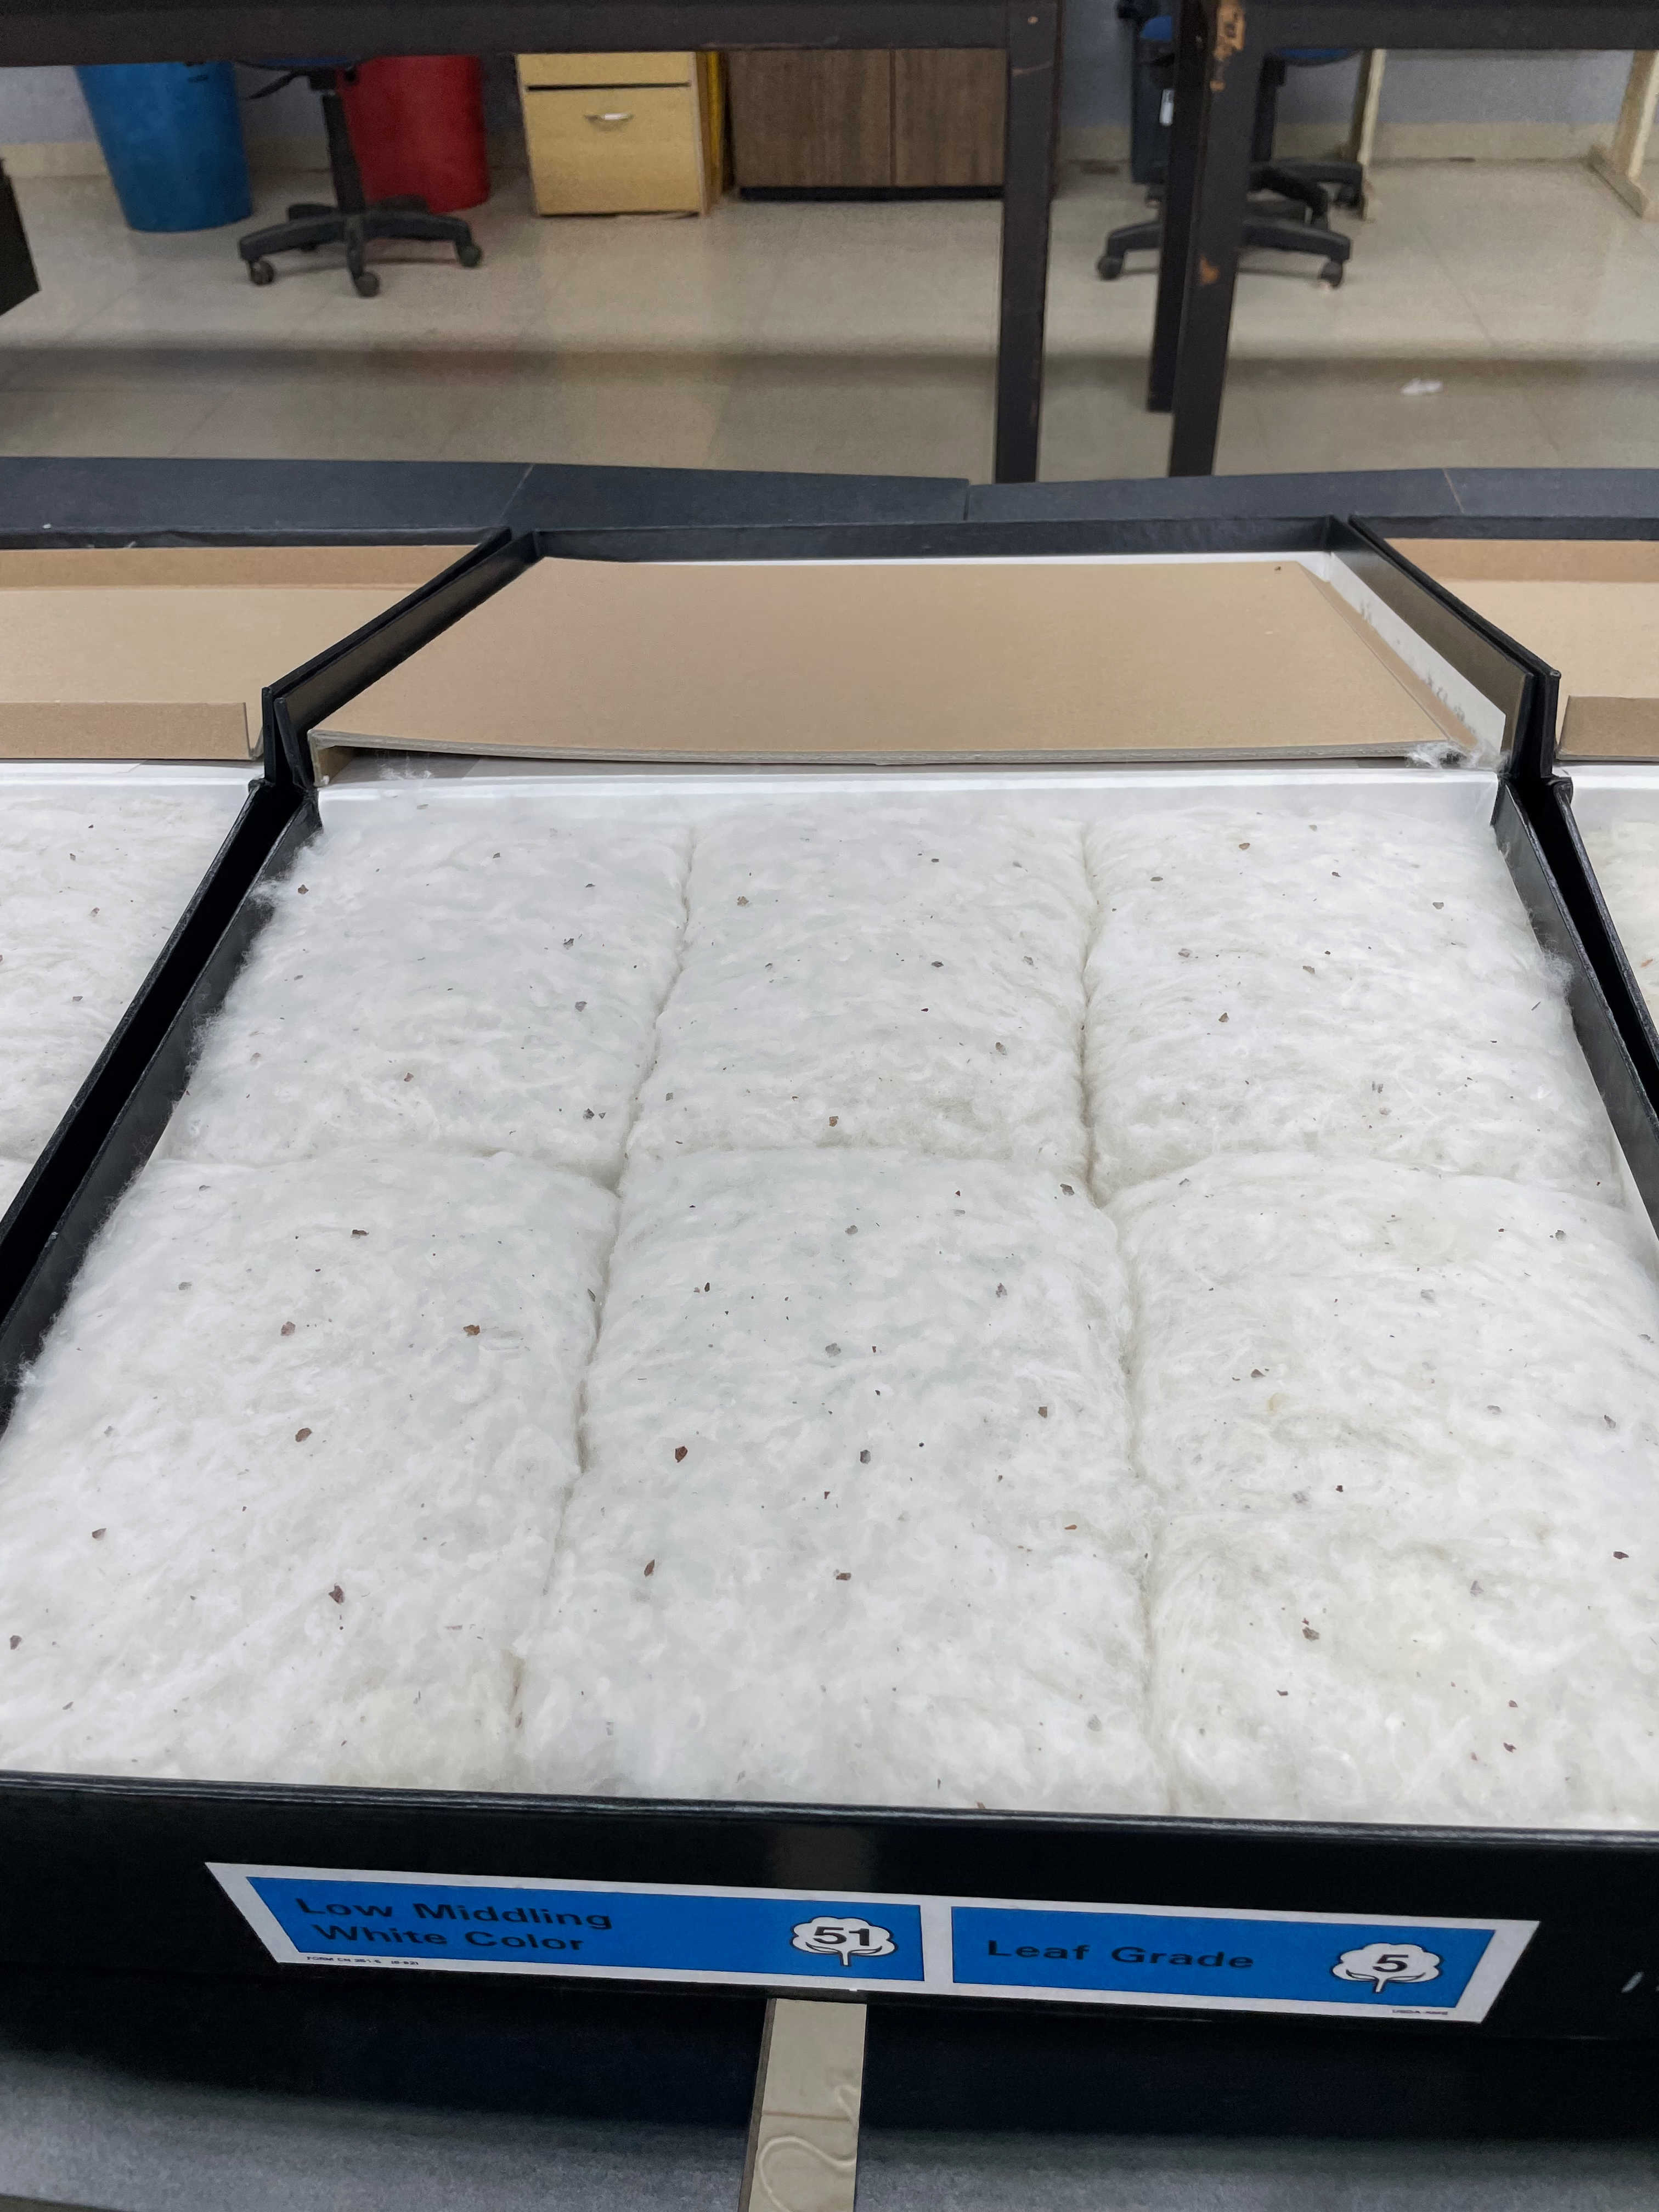
\includegraphics[trim={0 0 0 5cm},clip, scale=.3]{images/padrao_fisico_universal.jpeg}
            \end{center}
            \legend{Fonte: Do Autor}
        \end{figure}

        O protocolo de análise é rigoroso e inicia-se pela calibração visual do técnico, que deve memorizar os padrões físicos antes de iniciar a classificação, podendo consultá-los sempre que necessário para evitar desvios de julgamento. O manuseio da amostra exige técnica específica: ela deve ser subdividida longitudinalmente em camadas, com cuidado para não descaracterizar sua estrutura. As duas faces com maior incidência de defeitos visíveis, são selecionadas e voltadas para cima para a avaliação final.

        Neste exame, o classificador julga simultaneamente múltiplos atributos qualitativos, conforme detalhado por \citeonline{abbade2014agro}:

        \begin{itemize}
            \item \textbf{Cor:} Avaliada pela combinação de matiz, saturação e brilho, sendo categorizada em classes (Branco, Ligeiramente Manchado, Manchado, Tingido e Amarelo);
            \item \textbf{Impurezas (Leaf Grade):} Quantificação visual de cascas, folhas, caules e outras matérias estranhas. O grau é atribuído em uma escala de 1 a 8, na qual 1 representa a amostra mais limpa e 8, a mais suja;
            \item \textbf{Preparação:} Identificação de defeitos oriundos do processo de beneficiamento, como a aspereza e a formação de nós de fibra (emaranhados de fibras);
            \item \textbf{Contaminações:} Presença de materiais não vegetais (plásticos, óleos, entre outros) que desclassificam o lote.
        \end{itemize}

        A determinação final do ``Tipo'' é uma composição entre o padrão de cor e o grau de folha, registrada no Laudo de Classificação (Tabela \ref{tab_tipo_cor}).

        Apesar da padronização dos critérios, a classificação visual possui limitações inerentes à percepção humana. \citeonline{matusiak2010important} argumentam que a análise sensorial é fortemente influenciada por fatores como cansaço visual, experiência do técnico e condições de iluminação. Essa subjetividade gera variabilidade nos resultados, tanto entre diferentes avaliadores quanto nas decisões do mesmo técnico em momentos distintos. Além disso, a dificuldade natural do olho humano em distinguir nuances sutis de cor ou quantificar impurezas milimétricas reforça a necessidade de sistemas de Visão Computacional, que oferecem a reprodutibilidade e a precisão objetiva exigidas pela indústria.

        \afterpage{%
    \clearpage% Flush earlier floats (otherwise order might not be correct)
    \thispagestyle{empty}% empty page style (?)
    \begin{landscape}% Landscape page
        \centering % Center table
        \begin{table}
            \centering
            \caption{Códigos dos tipos de Cor, Classes de Cor ou Grau de Cor do Algodão Upland}
            \begin{tblr}{
                width = \linewidth,
                colspec = {Q[l,m,400]Q[c,m,180]Q[c,m,220]Q[c,m,180]Q[c,m,220]Q[c,m,180]},
                row{1} = {font=\bfseries},
                vline{2-6} = {-}{},
                hline{3-9} = {-}{},
                hline{1-2,10} = {2pt}
              }
                                                                                  & Branco & Ligeiramente Creme & Creme & Avermelhado & Amarelado \\
              Cor Boa Média - GM (Good Middling)                         & 11              & 12                          & 13             & -                    & -                  \\
              Cor Estritamente Média-SM (Strict Middling)                & 21              & 22                          & 23             & 24                   & 25                 \\
              Cor Média-M (Middling)                                     & 31              & 32                          & 33             & 34                   & 35                 \\
              Cor Estritamente Abaixo da Média-SLM (Strict Low Middling) & 41              & 42                          & 43             & 44                   & -                  \\
              Cor Abaixo da Média-LM (Low Middling)                      & 51              & 52                          & 53             & 54                   & -                  \\
              Cor Estritamente Boa Comum-SGO (Strict Good Ordinary)      & 61              & 62                          & 63             & -                    & -                  \\
              Cor Boa Comum-GO (Good Ordinary)                           & 71              & -                           & -              & -                    & -                  \\
              Abaixo de Padrão                                           & 81              & 82                          & 83             & 84                   & 85                 
              \end{tblr}
        \label{tab_tipo_cor}
        \end{table}
    \end{landscape}
    \clearpage
}

    \subsubsection{O Impacto do Viés Subjetivo Humano na Definição do Padrão de Referência (\textit{Ground Truth})}
    \label{sec:vies_humano_gt}

        A qualidade preditiva de qualquer sistema de visão computacional profundo é intrinsecamente
        limitada pela fidelidade do sinal de rotulagem utilizado como padrão de referência
        (\textit{ground truth}). Para além dos fatores já discutidos --- cansaço visual, experiência
        do técnico e condições de iluminação --- a subjetividade da tipagem visual regida pela
        Instrução Normativa nº 24/2016 do MAPA é também influenciada por um viés cognitivo-comercial
        do avaliador, resultando em uma concordância entre classificadores humanos experientes que é
        historicamente instável, tanto entre diferentes avaliadores quanto nas decisões do mesmo
        técnico em momentos distintos \cite{matusiak2010important, fisher2023aiassisted}.

        Uma vez que o conjunto de dados de referência utilizado nesta dissertação foi rotulado a
        partir dos laudos de classificação visual humana da algodoeira parceira em Sapezal, Mato
        Grosso (Seção \ref{sec:conjunto_dados}), as inconsistências inerentes ao julgamento humano
        atuam como um ruído estocástico incorporado aos próprios rótulos de treinamento. Esse fator
        impõe um limite superior (\textit{upper bound}) ao desempenho teórico absoluto das redes
        neurais avaliadas, uma vez que os modelos são forçados a mapear fronteiras de decisão
        qualitativas e fluidas que, por vezes, carecem de consistência física estrita.

        \clearpage

    \subsubsection{A Classificação Instrumental (HVI)}

        Paralelamente à análise visual, a segunda amostra de trabalho é destinada à classificação instrumental. Diferente da avaliação humana, essa etapa exige rigoroso controle ambiental: as amostras devem permanecer em repouso em bandejas teladas por, no mínimo, 24 horas em laboratório climatizado (temperatura e umidade controladas) para atingir o equilíbrio de umidade com o ambiente, garantindo a reprodutibilidade das leituras físicas.

        A análise é realizada em equipamentos de alto volume conhecidos como HVI, calibrados diariamente com padrões internacionais do USDA. A Figura \ref{fig_hvi_maquina} apresenta o modelo Uster HVI 1000, amplamente adotado pela indústria têxtil.

        \begin{figure}[H]
            \caption{\label{fig_hvi_maquina}Equipamento Uster HVI 1000}
            \begin{center}
                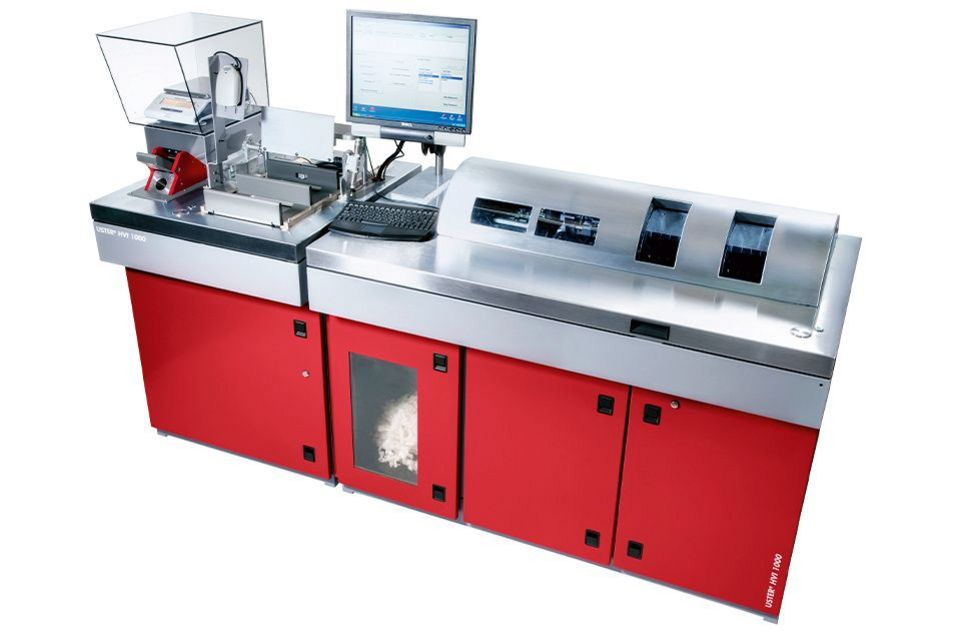
\includegraphics[trim={0 0 0 0},clip, scale=.3]{images/hvi_maquina.jpg}
            \end{center}
            \legend{Fonte: \cite{uster2024hvi}}
        \end{figure}

        O protocolo operacional do HVI automatiza a mensuração de múltiplas propriedades físicas. O teste de \textit{Micronaire} é realizado em um único corpo de prova por meio da compressão de massa de fibras, enquanto os demais parâmetros de comprimento e resistência são obtidos por meio de pentes óticos e garras mecânicas em dois corpos de prova por amostra, gerando uma média do lote.

        Os principais parâmetros fornecidos no laudo técnico são:

        \begin{itemize}
            \item \textbf{Comprimento da Fibra (UHML):} Comprimento médio da metade superior das fibras.
            \item \textbf{Índice de Uniformidade do Comprimento da Fibra (\%UI):} Relação entre o comprimento médio total das fibras e o comprimento médio das fibras mais longas.
            \item \textbf{Resistência ou Tenacidade da Fibra (Str):} Medida da força necessária para romper as fibras, expressa em gf/tex.
            \item \textbf{Alongamento à Rotura da Fibra (\%Elg):} Percentual de extensão que a fibra suporta antes de romper.
            \item \textbf{Micronaire da Fibra (Mic):} Combinação de finura e maturidade da fibra.
            \item \textbf{Grau de Reflectância (\%Rd):} Nível de luminosidade e cor branca refletida pelas fibras.
            \item \textbf{Grau de Amarelamento (+b):} Índice que expressa o nível de amarelamento da fibra.
            \item \textbf{Índice de Fibras Curtas (\%SFI):} Percentual de fibras com comprimento inferior a 0,50 polegadas.
            \item \textbf{Índice de Consistência da Fiação (SCI):} Valor calculado com base nas propriedades físicas das fibras e sua correlação com a performance de fiação.
        \end{itemize}

        Embora o HVI tenha trazido objetividade às transações comerciais, ele apresenta limitações críticas sob a ótica da classificação final. Além do alto custo de aquisição e manutenção \cite{cottonbrazil2021}, o equipamento fornece métricas baseadas em médias globais da amostra. Isso significa que, embora o HVI quantifique com precisão a área total de impurezas, ele não captura a percepção visual holística, como a distribuição espacial da sujeira, a textura e o contraste com a fibra, utilizada pelos classificadores humanos para determinar o ``Tipo'' comercial. Essa lacuna de percepção é justamente o nicho onde sistemas de visão computacional baseados em aprendizado profundo se destacam, pois são capazes de correlacionar padrões visuais complexos diretamente com os graus de qualidade padronizados, oferecendo uma alternativa automatizada e consistente à subjetividade humana.

    \subsubsection{A Relação entre o Visual e o Instrumental}

        A integração entre a subjetividade da análise visual e a objetividade instrumental baseia-se historicamente nos estudos de \citeonline{nickerson1958grade}. Buscando traduzir a percepção humana para grandezas físicas mensuráveis, os autores desenvolveram o colorímetro Nickerson-Hunter, estabelecendo as bases para o atual diagrama de cores utilizado pelo sistema HVI.

        Conforme ilustrado na Figura \ref{fig_hvi_color_chart}, a relação é estabelecida em um plano bidimensional no qual:

        \begin{itemize}
            \item O eixo vertical (\textbf{\%Rd}) representa a \textbf{Reflectância} (brilho), correlacionando-se com a escala de cinzas (do branco ao cinza escuro);
            \item O eixo horizontal (\textbf{+b}) representa o \textbf{Grau de Amarelamento}, indicando a saturação da cor amarela na fibra.
        \end{itemize}

        As interseções desses valores formam clusters que correspondem às classes visuais tradicionais (por exemplo, \textit{Middling}, \textit{Strict Low Middling}). Dessa forma, o HVI consegue converter leituras sensoriais em uma ``nota'' comercial compatível com o julgamento humano.

        \clearpage
        \begin{figure}[H]
            \caption{\label{fig_hvi_color_chart}Diagrama de Cores relacionando parâmetros físicos (\%Rd e +b) com a classificação visual.}
            \begin{center}
                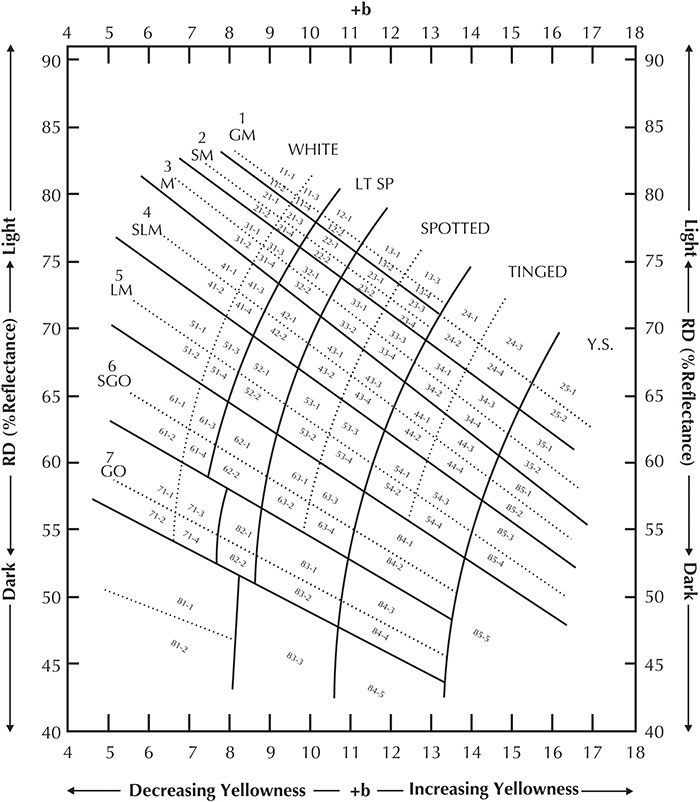
\includegraphics[trim={0 0 0 0},clip, scale=.5]{images/hvi_color_chart.jpg}
            \end{center}
            \legend{Fonte: \citeonline{cottoninc2024hvicolor}}
            % \nota{}
        \end{figure}

        Entretanto, essa correlação robusta observada na análise de cor não se verifica com a mesma eficácia para os parâmetros de impurezas e preparação. Enquanto o HVI mensura a sujeira por contagem de partículas e área ocupada, o classificador humano avalia a aparência geral, considerando o contraste, o tamanho e a natureza do resíduo (folha, casca ou caule). Estudos indicam que a correlação entre o ``Grau de Folha'' visual e a leitura de ``\%Area'' do HVI pode ser baixa em lotes com sujeira heterogênea.

        Essa discrepância evidencia uma lacuna tecnológica: o instrumento é preciso na física (cor), mas limitado na interpretação de padrões complexos (sujeira e textura). É nesse cenário que se insere a proposta desta dissertação: utilizar técnicas de visão computacional para reproduzir a percepção cognitiva humana, buscando uma classificação de qualidade que considere não apenas a estatística da sujeira, mas sua morfologia e distribuição visual na pluma.
